\section{Context}

\begin{frame}{Context}

Thin strip graphs are graphs that lie between the classes of unit disk graphs and unit interval graphs.
\vfill
\pause
\begin{figure}
\centering
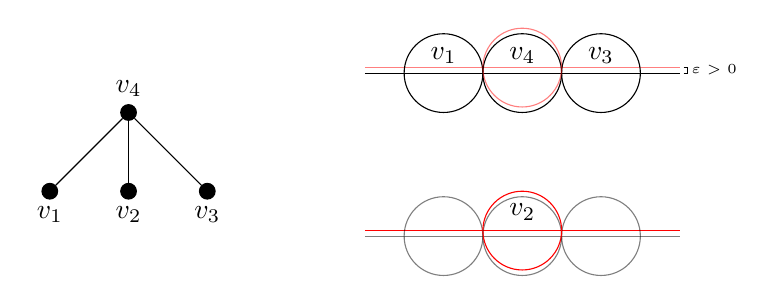
\begin{tikzpicture}[scale=1]

\draw (-2,0) -- (2,0);
\draw[red ,opacity = 0.5] (-2,0.07) -- (2,0.07);
\draw  (-1,0) circle [radius=0.5];
\draw[color=black] (-1,0.2265) node {$v_1$};
\draw  (0,0) circle [radius=0.5];
\draw[color=black] (0,0.2265) node {$v_4$};
\draw  (1,0) circle [radius=0.5];
\draw[color=black] (1,0.2265) node {$v_3$};

\draw[red, opacity = 0.5] (0,0.07) circle [radius=0.5];
\draw[color=black] (2.4386,0.0367) node {\tiny $\varepsilon > 0$};

% lines to describe distance (epsilon)
\draw[very thin] (2.1,0.07) -- (2.1,0);
\draw[very thin] (2.05,0.07) -- (2.1,0.07);
\draw[very thin] (2.05,0) -- (2.1,0);

\draw[opacity = 0.5] (-2,-2.07) -- (2,-2.07);
\draw[red] (-2,-2) -- (2,-2);
\draw[opacity = 0.5]  (0,-2.07) circle [radius=0.5];
\draw[opacity = 0.5]  (1,-2.07) circle [radius=0.5];
\draw[opacity = 0.5]  (-1,-2.07) circle [radius=0.5];
\draw[red] (0,-2) circle [radius=0.5];
\draw[color=black] (0,-1.765) node {$v_2$};

\node[draw,circle,inner sep=2pt,fill,label distance=1cm] (v1) at (-5,-0.5) {};
\draw[color=black] (-5,-0.2) node {$v_4$};
\node[draw,circle,inner sep=2pt,fill,label distance=1cm] (v3) at (-5,-1.5) {};
\draw[color=black] (-5,-1.8) node {$v_2$};
\node[draw,circle,inner sep=2pt,fill,label distance=1cm] (v2) at (-6,-1.5) {};
\draw[color=black] (-4,-1.8) node {$v_3$};
\node[draw,circle,inner sep=2pt,fill,label distance=1cm] (v4) at (-4,-1.5) {};
\draw[color=black] (-6,-1.8) node {$v_1$};
\draw  (v1) edge (v2);
\draw  (v1) edge (v3);
\draw  (v1) edge (v4);
\end{tikzpicture}
\label{fig:thinK13}
\end{figure}

\end{frame}

\begin{frame}{Context}
  The research in this paper is based on three papers.

  \begin{itemize}[<+->]
    \item T. Hayashi, A. Kawamura, Y, Otachi, H. Shinohara and K. Yamazaki. Thin Strip Graphs. Discrete Applied Mathematics. 2017.
    \item F. Joos. A Characterization of Mixed Unit Interval Graphs. Journal of Graph Theory. 2014.
    \item H. Breu. Algorithmic aspects of constrained unit disk graphs. Thesis, 1996
  \end{itemize}

\end{frame}
